\section{RISC-V}

A RISC-V é uma \gls{isa} baseada nos princípios \gls{risc}. Diferentemente de arquiteturas proprietárias,
a RISC-V possui uma especificação aberta e livre de \textit{royalties}, o que permite sua utilização tanto em contextos acadêmicos quanto em aplicações
comerciais.

Essa \gls{isa} define um conjunto básico de instruções, responsável pelas funcionalidades essenciais do processador. No entanto, sua
principal característica é a modularidade, permitindo que diferentes extensões sejam incorporadas conforme as necessidades da plataforma.
Dessa forma, é possível adaptar a arquitetura para cenários variados, desde sistemas embarcados com restrições de recursos até sistemas de
alto desempenho.

\subsection{Extensões Básicas}

\begin{description}

\item[I]
Adiciona suporte às instruções básicas de operações com números inteiros. Conforme descrito em~\cite{isa-riscv}, essa extensão deve estar
presente em qualquer implementação RISC-V, pois define as operações fundamentais de aritmética e manipulação de registradores.

\item[Zicsr]
Adiciona suporte às instruções de acesso e manipulação de \glspl{csr}.

\item[H]
Adiciona suporte ao modo H (Hipervisor).

\item[S]
Adiciona suporte ao modo S (Supervisor).

\item[M]
Adiciona suporte a operações de multiplicação e divisão de números inteiros.

\item[A]
Adiciona suporte a operações atômicas em memória.

\item[F]
Adiciona suporte a números em ponto flutuante de precisão simples (32 bits).

\item[D]
Adiciona suporte a números em ponto flutuante de precisão dupla (64 bits).

\item[C]
Adiciona suporte a instruções comprimidas de 16 bits.

\item[V]
Adiciona suporte a operações vetoriais para \gls{simd}.

\item[B]
Adiciona suporte à manipulação de bits em hardware, otimizando operações bit a bit.

\item[G]
Aglomerado geral de extensões (*General Purpose*) que inclui I, M, A, F, D e as extensões de controle Zicsr e Zifencei.

\end{description}

\subsection{Níveis de Privilégio}

Assim como a maior parte das arquiteturas modernas, a RISC-V utiliza um modelo hierárquico de privilégios para garantir a segurança e a estabilidade do sistema.
Esses níveis determinam quais operações e recursos de hardware podem ser acessados em cada contexto de execução. Os modos implementados em uma plataforma dependem
diretamente das extensões suportadas, estruturando-se tipicamente em três cenários principais:

\begin{itemize}

\item \textbf{Sem a extensão S:} Utiliza apenas o modo \textit{Machine} e o modo \textit{User}, indicado para sistemas embarcados mais simples e sem suporte a sistemas operacionais baseados em supervisor.
    \begin{figure}[H]
    \centering
    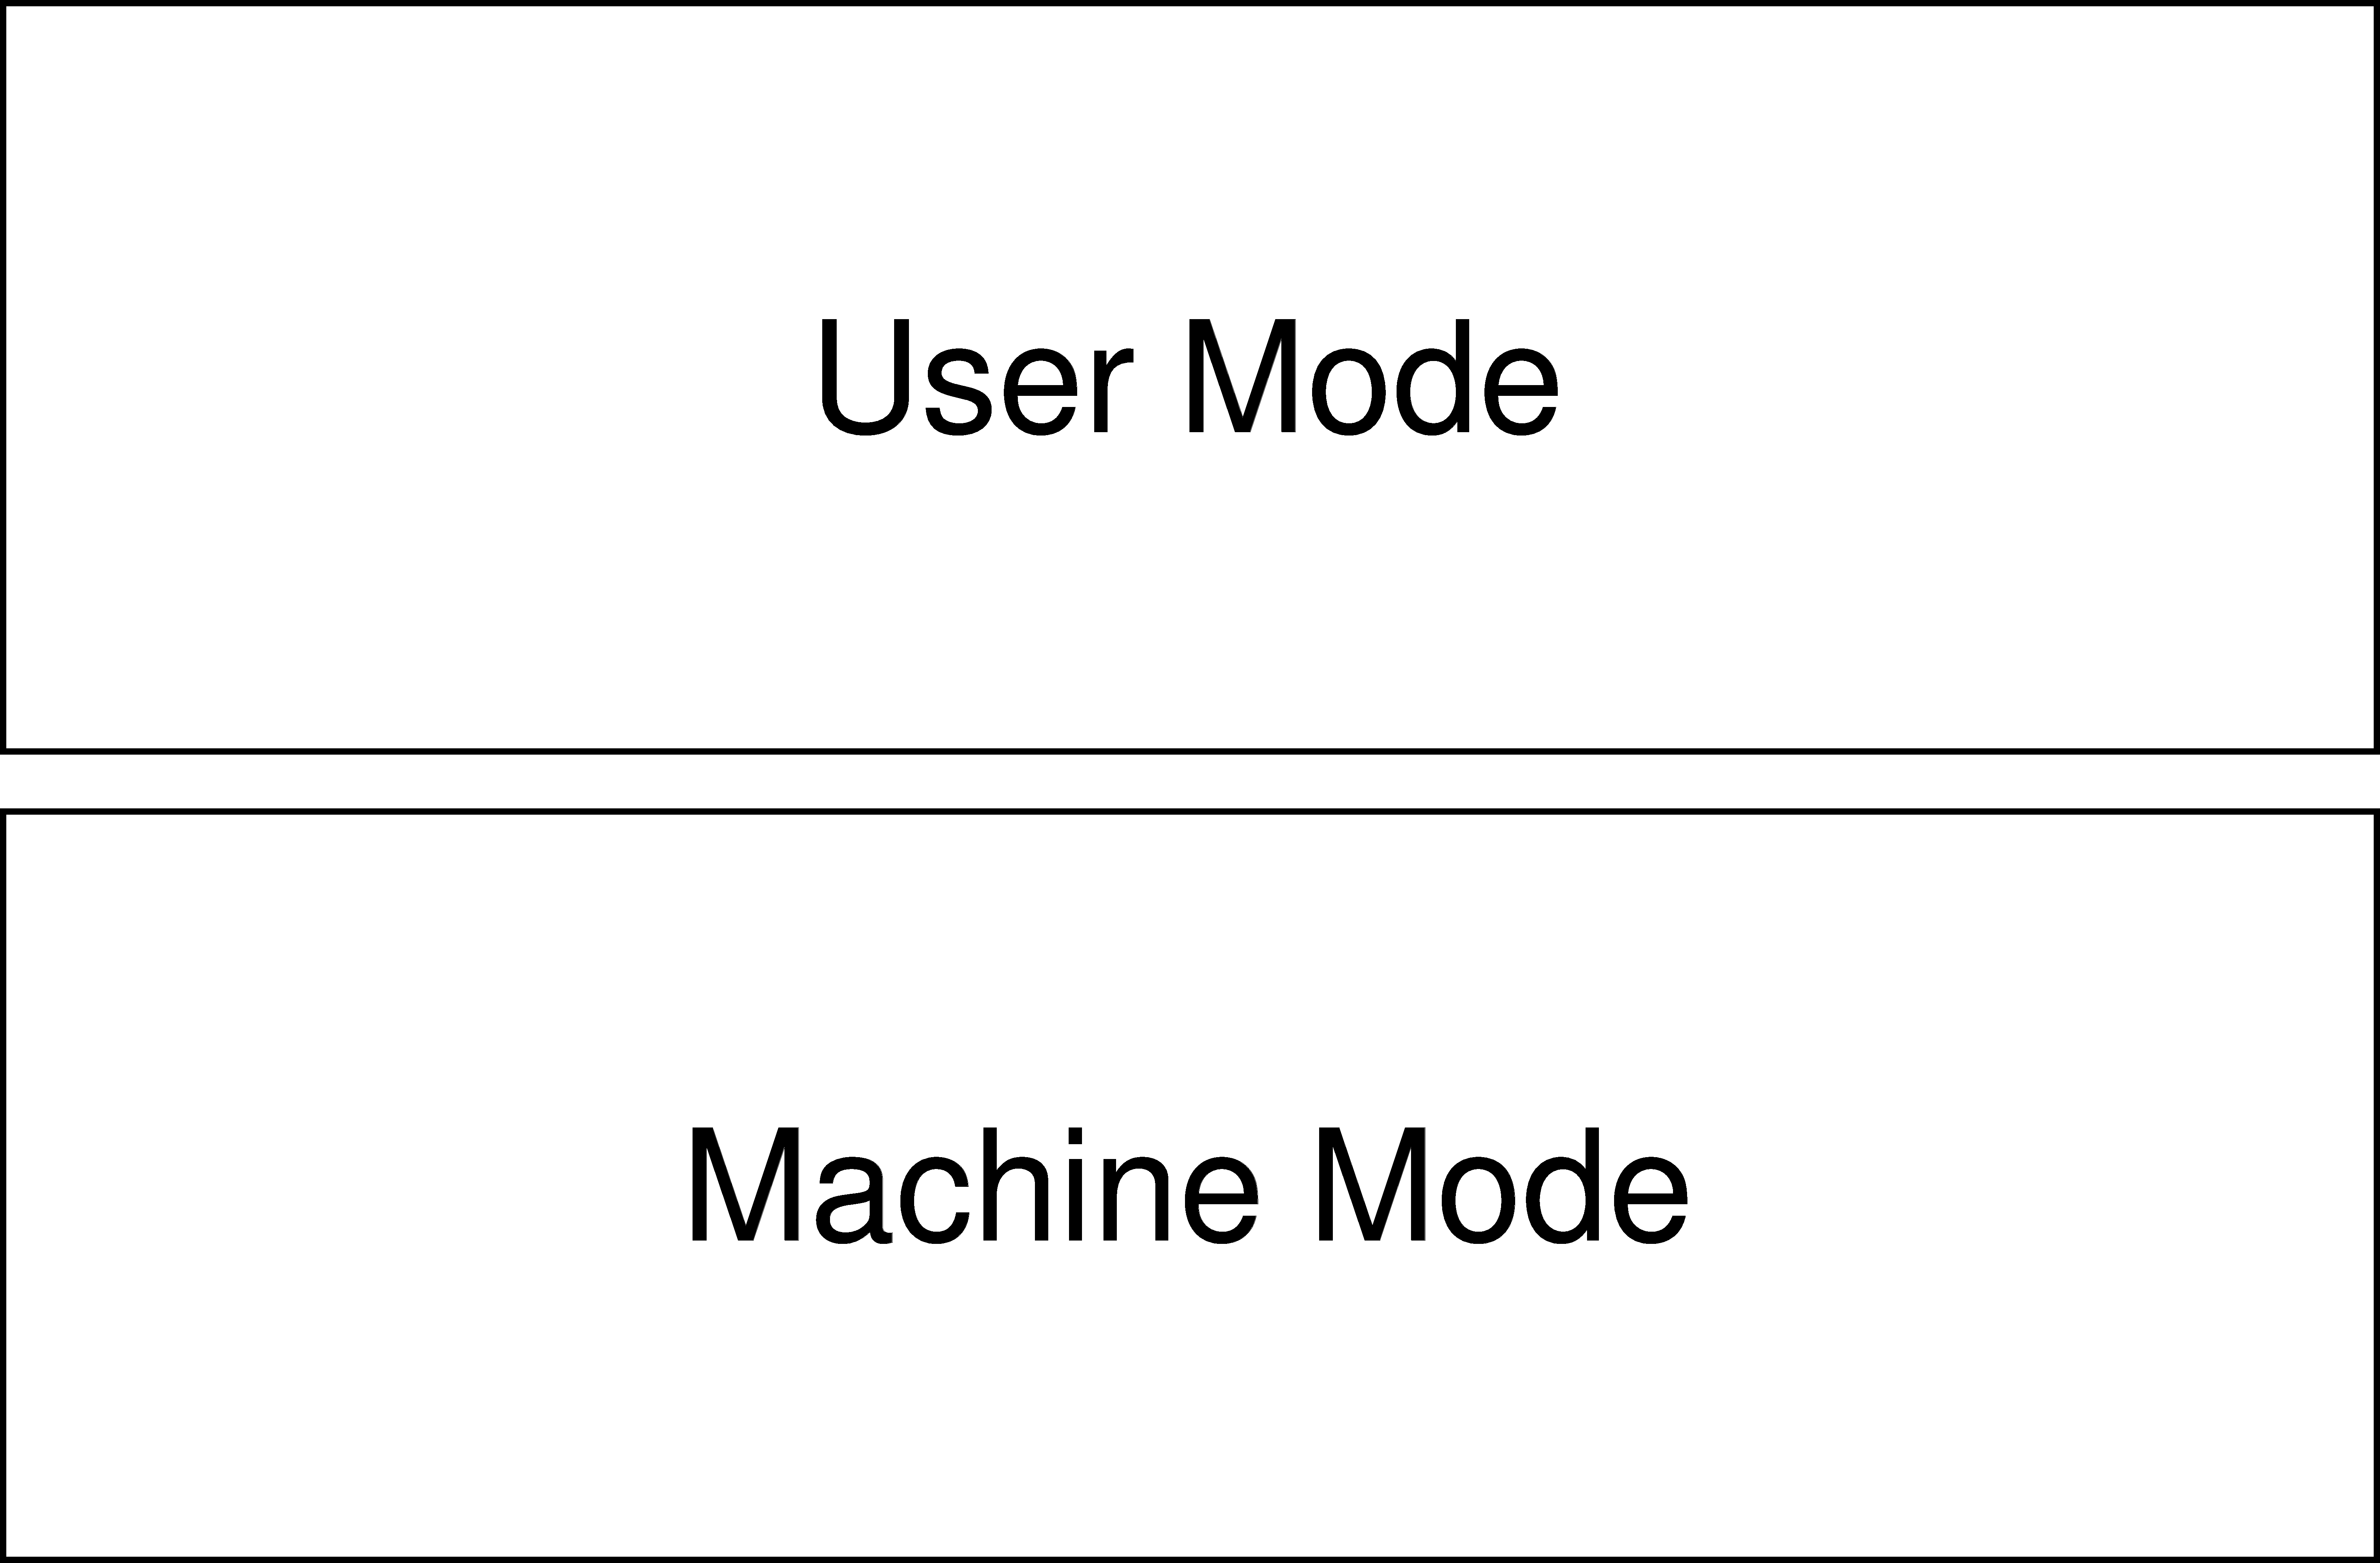
\includegraphics[width=0.3\textwidth]{images/MachineModeUserMode.pdf}
    \caption{Arquitetura de Privilégios RISC-V Sem Modo Supervisor}\label{fig:machine-mode-user-mode}
    \end{figure}

\item \textbf{Com a extensão S:} Adiciona o modo \textit{Supervisor}, permitindo a execução de sistemas operacionais completos que exigem isolamento entre o kernel e as aplicações de usuário.
    \begin{figure}[H]
    \centering
    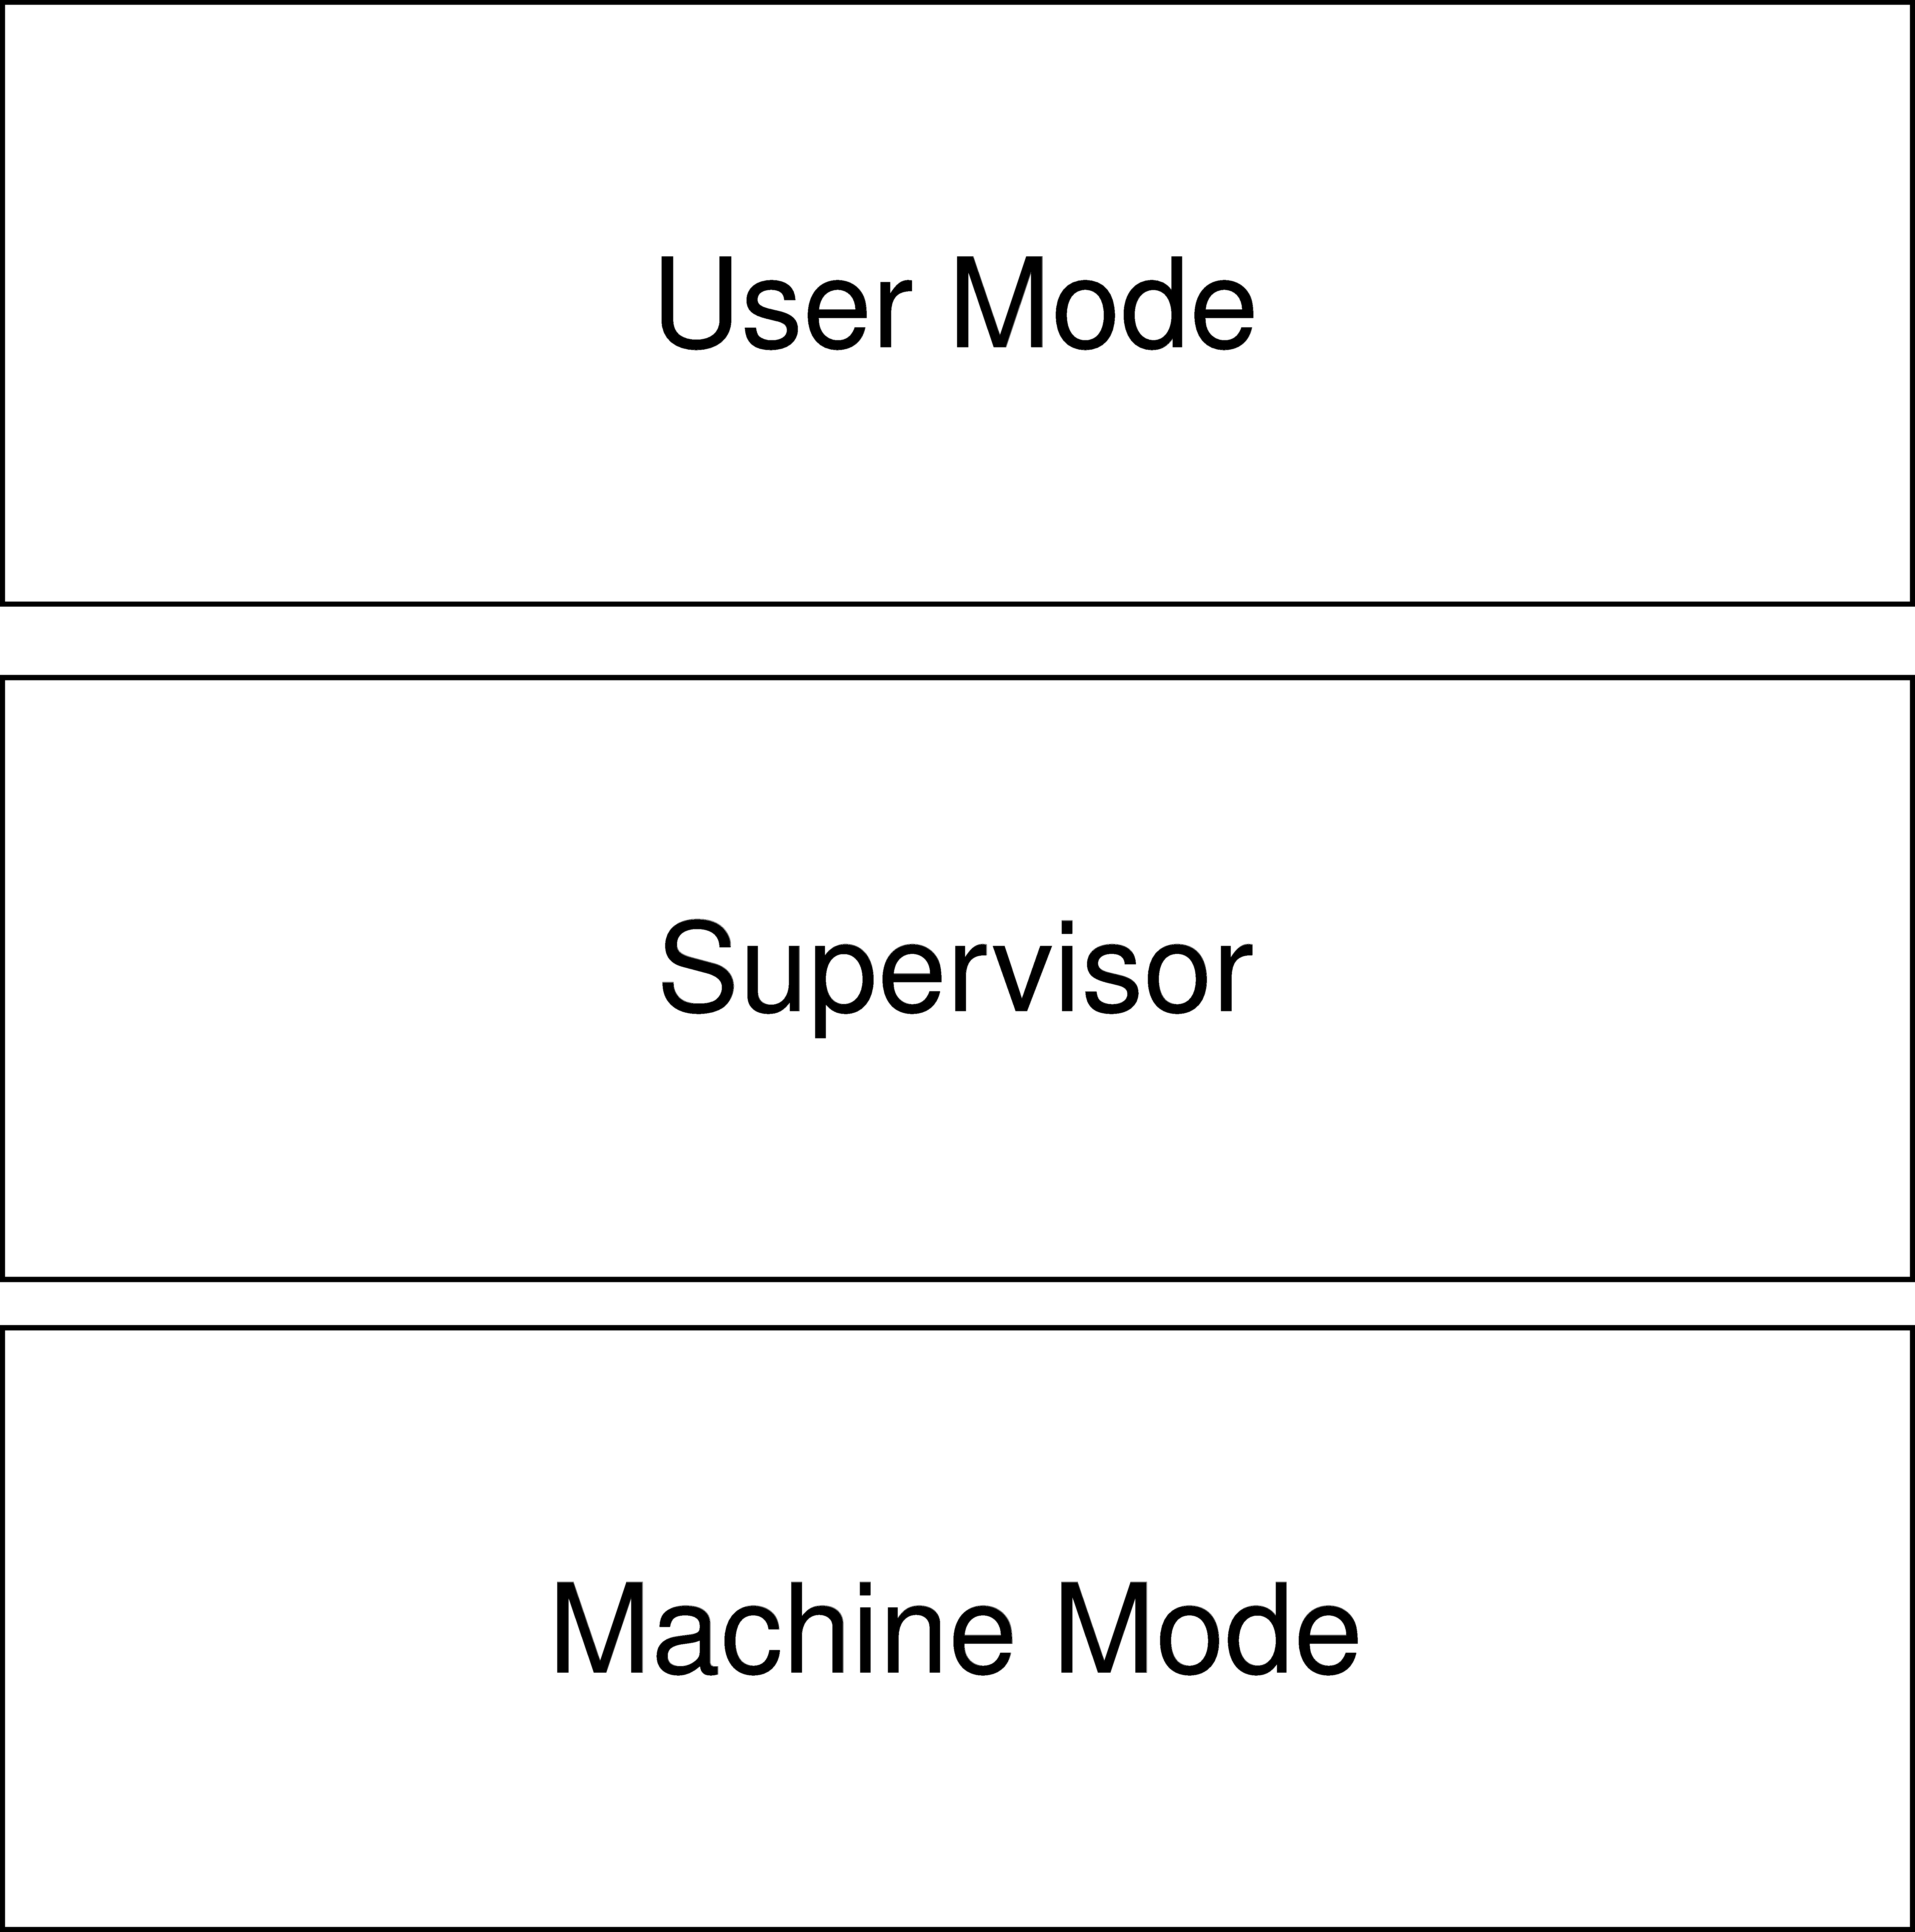
\includegraphics[width=0.3\textwidth]{images/SupervisorMode.pdf}
    \caption{Arquitetura de Privilégios RISC-V Com Modo Supervisor}\label{fig:machine-mode-user-mode-supervisor-mode}
    \end{figure}

\item \textbf{Com a extensão H:} Introduz o suporte aos modos \textit{Virtual User} e \textit{Virtual Supervisor}, estendendo os modos de privilégio para permitir a execução de hipervisores modernos.
    \begin{figure}[H]
    \centering
    \includegraphics[width=0.3\textwidth]{images/HypervisorMode.pdf}
    \caption{Arquitetura de Privilégios RISC-V Com Extensão H}\label{fig:riscv-hypervisor-mode}
    \end{figure}

\end{itemize}

\subsection{Registradores de Controle}

Os \glspl{csr} são registradores especiais utilizados para controlar e monitorar o funcionamento do processador. Eles armazenam informações essenciais relacionadas
ao estado da máquina, ao tratamento de exceções e interrupções, à configuração de privilégios e ao controle de funcionalidades específicas da arquitetura.

Esses registradores são organizados de forma segregada por nível de privilégio, sendo que cada nível dispõe do seu próprio conjunto de \glspl{csr}.
Esse isolamento é fundamental para a segurança e a integridade do sistema, pois garante uma política rígida de acessibilidade: um nível de privilégio só
pode acessar seus próprios registradores ou aqueles pertencentes a níveis menos privilegiados. Qualquer tentativa de acesso indevido a um \gls{csr} de um nível mais privilegiado 
resulta em uma exceção de instrução ilegal, impedindo que código menos privilegiado interfira diretamente nas camadas críticas do sistema.

Os principais \glspl{csr} são:

\begin{itemize}
    \item \texttt{mhartid}: mantém o identificador único de cada núcleo da CPU;\@
    \item \texttt{mstatus} e \texttt{mstatush}: mantêm os principais bits de configuração relacionados à arquitetura;
    \item \texttt{mtvec}: armazena o endereço base do vetor de manipuladores de exceções e interrupções no modo \textit{Machine};
    \item \texttt{mepc}: guarda o endereço da instrução que causou a exceção ou interrupção no modo \textit{Machine};
	\item \texttt{mcause}: armazena a causa de uma instrução ou exceção no modo \textit{Machine};
    \item \texttt{mtval}: armazena dados adicionais de uma exceção no modo \textit{Machine};
    \item \texttt{mscratch}: registrador temporário de rascunho usado para salvar ponteiros de contexto durante manipuladores no modo \textit{Machine};
    \item \texttt{mideleg} e \texttt{medeleg}: configuram a delegação de interrupções e exceções do modo \textit{Machine} para modos de menor privilégio;
    \item \texttt{mip}: mantém as interrupções atualmente pendentes;
    \item \texttt{mie}: mantém as interrupções atualmente habilitadas;
    \item \texttt{sstatus}: versão restrita e visível do registrador de status para o modo \textit{Supervisor};
    \item \texttt{stvec}: armazena o endereço base do manipulador de \textit{traps} no modo \textit{Supervisor};
    \item \texttt{sepc}: guarda o endereço da instrução que causou a exceção ou interrupção no modo \textit{Supervisor};
    \item \texttt{scause}: armazena a causa da interrupção ou exceção no modo \textit{Supervisor};
    \item \texttt{stval}: guarda informações adicionais relativas à exceção ocorrida no modo \textit{Supervisor};
    \item \texttt{sscratch}: registrador de rascunho temporário do modo \textit{Supervisor};
    \item \texttt{sip}: correspondente do modo \textit{Supervisor} ao \texttt{mip};
    \item \texttt{sie}: correspondente do modo \textit{Supervisor} ao \texttt{mie};
    \item \texttt{satp}: controla a tradução de endereços virtuais e a paginação da memória no modo \textit{Supervisor}.
\end{itemize}

\subsection{\gls{clint}}

O \gls{clint} é o mecanismo responsável por gerenciar interrupções locais — especificamente as de software e de temporização — em plataformas RISC-V.

Para a gestão de tempo, o \gls{clint} possui dois registradores centrais: \texttt{mtime} e \texttt{mtimecmp}. O \texttt{mtime} funciona como a referência temporal principal da arquitetura,
mantendo o \gls{so} ciente da passagem do tempo. O \texttt{mtimecmp}, por sua vez, determina o momento em que uma interrupção de temporização deve ser disparada:
quando o valor de \texttt{mtime} torna-se maior ou igual ao de \texttt{mtimecmp}, o \gls{clint} sinaliza o bit de interrupção temporal no registrador \gls{mip}.

Em relação às interrupções de software, o \gls{clint} disponibiliza um registrador \gls{msip} mapeado em memória para cada núcleo. Dessa forma, um núcleo pode disparar
uma interrupção de software em outro ativando o bit zero do registrador \gls{msip} pertencente ao núcleo de destino.

\subsection{\gls{plic}}

O funcionamento do \gls{plic} baseia-se na centralização e priorização de solicitações provenientes de periféricos externos. Quando uma interrupção atende aos requisitos
de habilitação e ao limiar de prioridade, o \gls{plic} notifica o núcleo ativando o bit correspondente de interrupção externa no registrador \gls{mip}, como \gls{meip} ou \gls{seip}.
A partir dessa notificação, para identificar e tratar a interrupção, o \gls{so} deve se comunicar ativamente com o \gls{plic}.

\subsection{Gerenciamento de Memória Virtual} 

A \gls{mmu} na arquitetura RISC-V é responsável por realizar a tradução de endereços virtuais em endereços físicos e por verificar as permissões de acesso à memória.
O mecanismo de tradução utilizado pelos sistemas operacionais é configurado por meio do registrador de controle \gls{satp}, disponível no modo \textit{Supervisor}.

Seu funcionamento baseia-se na paginação da memória, na qual os endereços virtuais são divididos em páginas, tipicamente com granularidade de 4,KiB. O \gls{so}
mantém tabelas de páginas que associam essas páginas virtuais a regiões da memória física e definem as permissões de acesso, como leitura, escrita e execução.
Dessa forma, quando um processo acessa um endereço virtual, a \gls{mmu} realiza a tradução correspondente e verifica se a operação solicitada é permitida.
Caso o endereço não esteja mapeado ou a operação viole as permissões estabelecidas, ocorre uma exceção de acesso à memória.

\subsection{Proteção de Memória Física}

Em sistemas que não possuem o modo supervisor --- ou como camada adicional de segurança ---, a arquitetura RISC-V emprega o mecanismo de \gls{pmp}.
Exclusivamente no modo \textit{Machine}, o firmware configura os registradores de \gls{pmp} para delimitar quais regiões da memória física podem ser acessadas pelos modos
\textit{User} e \textit{Supervisor}, assegurando o isolamento por hardware mesmo na ausência ou antes da inicialização de uma \gls{mmu}.

Para gerenciar essas regras, o mecanismo baseia-se em dois tipos de registradores: os registradores de configuração --- \textit{pmpcfg}, que definem as permissões de
acesso --- leitura, escrita e execução, o modo de pareamento de endereços e o bit de travamento para cada entrada; e os registradores de endereço --- \textit{pmpaddr},
que armazenam os endereços de referência ou parâmetros empregados pelo hardware para delimitar o tamanho e os limites das regiões protegidas.

O mecanismo de \gls{pmp} definido pela \gls{isa} da RISC-V possui três modos ativos de pareamento de endereços:

\begin{itemize}
    \item \textbf{\gls{tor}:} define uma faixa contínua de memória onde o registrador $\textit{pmpaddr}_i$ atua como o limite superior --- exclusivo --- e
        o registrador anterior $\textit{pmpaddr}_{i-1}$ atua como o limite inferior --- inclusivo. Para a primeira entrada ($i=0$), o limite inferior é considerado o
        endereço \textit{0$\times$0};
    \item \textbf{\gls{na4}:} mapeia um bloco fixo de exatamente 4 bytes apontado diretamente pelo registrador \textit{pmpaddr};
    \item \textbf{\gls{napot}:} define blocos com tamanhos que são potências de 2. O tamanho e o alinhamento da região são codificados nos bits menos significativos do próprio registrador \textit{pmpaddr}.
\end{itemize}

\subsection{Extensão H}

A extensão H introduz suporte nativo à virtualização em nível de hardware na arquitetura RISC-V. O principal objetivo dessa extensão é permitir a execução eficiente de um \gls{vmm}.
Para viabilizar esse isolamento e controle, a extensão H expande o modelo de privilégios da arquitetura, adicionando novos modos de execução:

\begin{itemize}
    \item \textbf{Virtual User:} modo no qual rodam as aplicações de usuário dentro do convidado.
    \item \textbf{Virtual Supervisor:} modo no qual o \gls{so} convidado é executado.
    \item \textbf{Hypervisor:} modo supervisor estendido, onde o hipervisor opera para gerenciar os recursos das \glspl{vm}.
\end{itemize}

\subsubsection{Tradução de Endereços em Dois Estágios}

Além dos novos modos de privilégio, a extensão H adiciona uma camada de tradução de memória para suportar a virtualização. Como múltiplos \glspl{so} convidados dependem da \gls{mmu} da plataforma
--- que normalmente seria controlada apenas pelo hipervisor ---, a arquitetura introduz os registradores \textit{vsatp} e \textit{hgatp} --- substitutos e complementos ao registrador padrão
\textit{satp} ---. Isso viabiliza uma tradução de endereços em dois estágios: o \textit{vsatp} mapeia os endereços virtuais do convidado para endereços físicos intermediários, enquanto o \textit{hgatp}
traduz esses endereços intermediários para a memória física real da máquina.

\begin{figure}[H]
\centering
\includegraphics[width=0.3\textwidth]{images/TwoStageMMU.pdf}
\caption{Tradução de Endereços em Dois Estágios da Extensão H}\label{fig:two-stage-mmu}
\end{figure}
